\documentclass[12pt,a4paper]{article}

\usepackage[utf8]{inputenc}
\usepackage[usenames,dvipsnames,table]{xcolor}
\usepackage{pgfplots}
\usepackage{amsfonts}
\usepackage{rotating}
\usepackage{pdfpages}
\frenchspacing
\usepackage{parskip}
\usepackage{graphicx}
\usepackage[sorting=none,citestyle=ieee,backend=biber]{biblatex}
\usepackage{pgfgantt}
\usepackage{float}
\usepackage{enumitem}
\usepackage[toc,page]{appendix}
\bibliography{progress-report}
\pgfplotsset{compat=1.11}

\title{Investigation Into the Use of Hardware Accelerators in Data Intensive Compute}
\author{CS310 Progress Report\\David Richardson, 1314918}
\date{November 2015}

\begin{document}
	\maketitle
	
	This document details the progress made in the investigation into the use of hardware accelerators in data intensive compute. Section \ref{sec:introduction} reintroduces the project and its aims as well as giving a summary of the project's objectives. Section \ref{sec:research_direction} identifies existing research in the project's problem domain. Section \ref{sec:benchmarking_progress} details the selection of the benchmarks to be used in the project, as well as any progress to the successful benchmarking of the cluster without hardware accelerators. Section \ref{sec:project_management} reiterates the approach to project management in the project specification, outlining any necessary changes that have been brought to light through the work so far. Section \ref{sec:further_work_project_extensions} outlines further work and extensions to the project. Finally, Section \ref{sec:conclusion} concludes by outlining the overall state of the project as well as reiterating the key points of the project's progression. More information about the specification of this project is available in the specification documentation in Appendix \ref{app:specification}.

	\section{Introduction}
	\label{sec:introduction}
	
	    Hardware accelerators provide the ability to offload a set of compute instructions from the CPU onto specialised hardware, designed to perform the computation faster and more efficiently than the CPU itself. These accelerators generally take the forms of General Purpose GPUs (GPGPUs) or Many Integrated Core (MIC) co-processors. With these hardware accelerators being included in an ever-increasing number of compute nodes within data centres, the chance to use them is increasing. However, the amount of research into their use within the paradigm of data intensive compute is underwhelming, despite their possible gains in power efficiency~\cite{energy-efficient-gpu} and speed~\cite{accelerating-matrix-product, quantitative-finance-gpu} over their general CPU counterparts. The integration of these hardware accelerators into the compute phases of data intensive workloads, such as MapReduce jobs, could provide benefits such as a reduction in the total compute time and power consumed by a workload. Other possible benefits involve a reduced need to scale outwards to cope with the Tera- or Petabyte scale data sets that have come about from the data avalanche in areas such as bioinformatics~\cite{big-data-biocuration}. These benefits are of interest to both academic and commercial applications, where it can reduce operational costs and reduce turn around time for compute workloads. Organisations such as that provide data-centric services such as Google or Facebook would also be able to enrich user experience with features that were not feasible due to slow compute times, also providing an increased value of service and profit.
	
	    \subsection{Project Aims}
	    \label{sub:project_aims}
	    
	        The underlying aim for this project is to test the use of GPGPUs and MIC co-processors in data intensive workloads to determine if their integration has significant improvements in compute and power consumption versus a CPU-only implementation. Their use has value for scientific and commercial areas, where a reduction in compute time will generally lead to a reduction in operational costs. It will also benefit infrastructure management companies such as Amazon, by increasing the performance per Watt of their compute nodes.
	        
	    \subsection{Summary of Objectives}
	    \label{sub:summary_of_objectives}
	    
	        The project has two main objectives that were outlined in the project specficiation documentation:
	        
	        \begin{enumerate}
	        \item To understand if current benchmarking suites are suitable for hardware accelerated data analytics clusters.
	        \item To determine if accelerators can be used within data analytics with little modification to current software stacks or algorithm implementations.
	        \end{enumerate}
	        
	        Where the notion of a `suitable' benchmark is a benchmark that tests a variety of work loads, makes use of any present hardware accelerators, and can be scaled in input data set size.
	    
    \section{Research Direction}
    \label{sec:research_direction}
    
        With the project introduced, the main aims for its research and the project's objectives all discussed, the area of related research is now considered.
    
        Research into the use of GPGPU and MIC co-processors within data intensive compute is limited at best, with very few technical reports or articles available.
        
        \subsection{Accelerating Breadth-First Search with Intel MIC Co-processors}
        \label{sub:accelerating_bfs_with_mic}
        
            Tao, Yutong, and Guang provide research into the application of the Intel MIC co-processor architecture to the Breadth-First Search (BFS) of a graph, a common data intensive compute workload. Their research considers both native and offload optimisations, outlining their optimisation procedures for both~\cite{mic-accelerate-bfs}. The native solution involves performing the BFS entirely on the co-processor and the optimisation techniques involved the exploitation of thread- and data-level parallelism. The offload solution will partition the tasks within the workload as well optimise communications between CPU and co-processor. They found that a native solution could run up to 3.4x faster on two Intel Xeon Phi Knight's Corner than when run on two Intel Xeon E5-2670. The offload algorithm results in a speed up of up to 1.67x. The offload algorithm also gains performance on larger graph sizes.
    
    \section{Benchmarking Progress}
    \label{sec:benchmarking_progress}
    
        With the nature of this project being mostly based around investigation and research, it is quite hard to measure its progress. However, it is possible to measure progress with regards to the timetable outlined in the project specification, where it lists the key phases to the project. The progress towards benchmark selection and execution is now to be discussed.
    
        \subsection{Benchmark Selection}
        \label{sub:benchmark_selection}
        
            There are a number of benchmarking suites available for use with compute clusters designed for the likes of data analytics or other data intensive compute workloads. For this project I will be selecting one benchmarking suite for use to compare the effect of the integration of hardware accelerators into them.
            
            Through my investigation into these benchmarks, a few observations have been made:
            
            \begin{enumerate}
            \item Most benchmarking suites come with their own scalable data generators.
            \item All benchmarking suites that have been considered are developed for MapReduce or similar compute workloads.
            \item All benchmarking suites investigated have not been built with the consideration for the use hardware accelerators.
            \end{enumerate}
            
            These observations can be used to conclude about objective 1 that was outlined in the project specification. This is that the current suite of benchmarks are not suitable for hardware accelerated data intensive compute clusters. This is due to the lack of consideration within the benchmarking suites, when developed, for the use of hardware accelerators like GPGPUs and MIC co-processors.
            
            With this in mind, the benchmarking suites that were considered are now discussed and compared.
    
            \subsubsection{Graph500}
            \label{ssub:graph500}
            
                The Graph500 is an initiative to establishe a set of large-scale benchmarks for data intensive applications, being backed by both academia and industry experts~\cite{graph500-intro}. At present, the Graph500 benchmark has only one workload that can be split into two kernels: generating a graph from an edge list, and a breadth-first search of the generated graph~\cite{graph500-spec}. The second kernel is measured in Traversed Edges per Second (TEPS), which provides a unit for comparison akin to LINPACK with Floating Point Operations per Second (FLOPS). The reference implementations provided by the Graph500 organisation are written in C and are available in sequential, OpenMP, XMT and MPI~\cite{graph500-reference-impl}.
        
            \subsubsection{BigDataBench}
            \label{ssub:bigdatabench}

            	BigDataBench is a data analytics benchmarking suite created at the ICT, Chinese Academy of Sciences, with backing from industry partners such as Huawei. The benchmarks in this suite abandon typical sequential and multithreaded workloads, that would typically use OpenMP or similar libraries, for scale-out~\cite{big-data-bench-home} workloads that are designed to better represent the distributed nature of data analytics. The benchmarks themselves in this suite are derived from a common subset of `dwarf' workloads, such as social network graph analysis or word multimedia analytics~\cite{dwarf-workloads-big-data}. These benchmarks are implemented using different technologies ranging from Apache Hadoop or Spark, to MySQL and C-based programs that use MPI for inter-node communications~\cite{big-data-bench-home}.
            
            \subsubsection{Intel HiBench}
            \label{ssub:intel_hibench}
            
            % Does similar workloads to BigDataBench.
            
            \subsubsection{Comparison and Conclusion}
            \label{ssub:comparison_and_conclusion}
            
            % All benchmarks haven't been developed with the prospect of hardware accelerators even being considered
            % BigDataBench has been selected, reasons explained here
            % HiBench uses different workloads are database-based and don't really map to GPU use cases.
            % Graph500 only uses OpenMP/MPI - doesn't consider MapReduce style workloads
            
        \subsection{Benchmark Running}
        \label{sub:benchmark_running}
        
        % Chiron has HDD/SSD storage - this could affect compute as data-intensive compute is IO bound
        % Compare InfiniBand to M.2/PCI-E 3.0 4x and SATA III standards to show storage IO is bottleneck instead of network throughput
        % Problems have been met mapping benchmark executables to Chiron's architecture (hadoop location, Chiron doesn't have some example jars, different storage architecture
    
    \section{Project Management}
    \label{sec:project_management}

        Having discussed the progress made in the project, attention is now turned to the project's management as well as where any changes to the project timetable or risk assessment will be considered.
    
        \subsection{Timetable}
        \label{sub:timetable}

            With Chiron remaining in a pre-production state, it is not without configuration errors and has a lack of user documentation. These issues will, as a result, add possible delays to the project as it moves forwards and the use of untested system components starts to occur. Fortunately the project timetable as given in the specification documentation has some contingencies built into it, in the form of task padding zones marked in red, as well as extra amount of time that allows the project to overrun without issue. Figure~\ref{fig:project-timetable} shows where the project is currently, with any complete tasks in violet. The overrun allowances for benchmark testing and accelerated benchmark testing and analysis have been extended, as well.

            \begin{sidewaysfigure}
                    \centering
                    \begin{ganttchart}[
                        x unit=6mm,
                        hgrid,
                        vgrid,
                        newline shortcut=true,
                        time slot format=simple,
                        bar/.append style={fill=green!15},
                        bar label node/.append style={align=left},
                        milestone inline label node/.append style={right=2mm},
                        milestone/.append style={fill=red},
                        today=9,
                        today offset=0.075,
                        today label=Current Week,
                        today label node/.append style={anchor=north west},
                        today label font=\itshape\color{red},
                        today rule/.style={draw=blue, ultra thick}
                    ]{1}{30}
                        \gantttitle{2015}{12}
                        \gantttitle{2016}{18} \\
                        \gantttitle{Time (in weeks)}{30} \\
                        \gantttitlelist{1,...,30}{1} \\
                        \ganttbar[bar/.append style={fill=violet!25}]{Benchmark selection}{1}{4} \ganttnewline
                        \ganttlinkedbar{Benchmark testing \ganttalignnewline
                            and analysis}{5}{8}
                        \ganttbar[bar/.append style={fill=red!25}]{}{9}{10} \ganttnewline
                        \ganttlinkedbar{Benchmark migration}{11}{14}
                        \ganttbar[bar/.append style={fill=red!25}]{}{15}{15} \ganttnewline
                        \ganttlinkedbar{Accelerated benchmark \ganttalignnewline
                            testing and analysis}{16}{17}
                        \ganttbar[bar/.append style={fill=red!25}]{}{18}{19}
                        \ganttlinkedmilestone[inline=true, milestone/.append style={fill=green}]{Research complete}{20} \ganttnewline[thick, black]
                        \ganttbar[bar/.append style={fill=violet!25}]{Project specification}{1}{2} 
                        \ganttmilestone[inline=true, milestone/.append style={fill=magenta}]{Submission}{2} \ganttnewline
                        \ganttbar[bar/.append style={fill=violet!25}]{Progress report}{6}{8}
                        \ganttmilestone[inline=true, milestone/.append style={fill=magenta}]{Submission}{8} \ganttnewline
                        \ganttbar[bar/.append style={fill=blue!15}]{Presentation prep.}{17}{21} 
                        \ganttlinkedmilestone[inline=true]{Presentation}{23} \ganttnewline
                        \ganttbar[bar/.append style={fill=blue!15}]{Final report}{11}{29}
                        \ganttlinkedmilestone{}{30}
                    \end{ganttchart}
                    \caption{Revised project timetable from week 1 term 1 to week 1 term 3}
                    \label{fig:project-timetable}       
                \end{sidewaysfigure}
        
        % Talk about where we are in the original timetable, as well as what changes may need to be made to accomodate for problems with Chiron
        
        \subsection{Risk Assessment}
        \label{sub:risk_assessment}

            In an ideal world, Chiron would have had user documentation generated and have been tested thoroughly. However, due to it being in pre-production mode, it is necessary to add the following risks to the risk matrix provided in the project specification documentation:

            \begin{itemize}
                \item A confuration error with Chiron's software stack.
                \item Software required to run a benchmark is not installed.
            \end{itemize}

            The amended risk matrix, with the risks mentioned above, is shown in figure~\ref{fig:risk_matrix}.

            \begin{figure}[H]
                \begin{center}
                    \begin{tabular}{| p{3cm} | l | l | p{4cm} |}
                        \hline
                        Risk & Severity & Likelihood & Mitigating Action(s) \\ \hline
                        Chiron unavailable & \cellcolor{red!15} Severe & \cellcolor{green!25} 0.01\% & Locate suitable replacement for use in testing --- replacement should have similar feature set to Chiron. \\ \hline
                        Benchmark code unavailable & \cellcolor{red!15} Severe & \cellcolor{yellow!15} 5\% & Check internet archives for possible location of older version. Find other suitable benchmarks. \\ \hline
                        Networking failure & \cellcolor{orange!15} Moderate-Severe & \cellcolor{yellow!15} 5\% & Temporarily locate to different area to use a different network. \\ \hline
                        Project leader falling ill & \cellcolor{yellow!15} Moderate & \cellcolor{orange!15} 10\% & Do work that can be done without further risk to health. \\ \hline
                        Configuration error with Chiron & \cellcolor{yellow!15} Moderate & \cellcolor{orange!15} 15\% & Report the bug using the Centre of Scientific Computing's BugZilla bug tracker. Attempt other work that doesn't depend on that particular software stack. \\ \hline
                        Required software for benchmark not installed & \cellcolor{red!15} Severe & \cellcolor{yellow!15} 5\% & Report the missing software to the Centre of Scientific Computing. In event of no resolution, another benchmark will be selected. \\ \hline
                    \end{tabular}
                \end{center}

                \caption{Risk matrix that associates possible risks with severity and mitigating actions}
                \label{fig:risk_matrix}
            \end{figure}
        
    \section{Further Work and Project Extensions}
    \label{sec:further_work_project_extensions}
    
        \subsection{Further Work}
        \label{sub:further_work}

            Benchmark suite selection for this project has been finalised, and the execution of those benchmarks is underway. With this in mind, there are two remaining tasks to be completed: Benchmark migration and accelerated benchmark testing and analysis. This section will detail the remaining tasks that are to be fulfilled as part of the project's completion.

                \subsubsection{Benchmark Migration}
                \label{sub:benchmark_migration}

                    The next step after the completion of benchmarking without accelerated codes is to then port these codes to the hardware accelerator platforms outlined within the project's specification documentation. This will involve identifying areas that are most suitable for application to the accelerator's architecture. After this identification process has finished, the accelerator's API calls will be injected into the codes and this code tested. Once the code has been migrated to the accelerator, re-integration into the MapReduce model will take place.

                \subsubsection{Accelerated Benchmark Testing and Analysis}
                \label{sub:accelerated_benchmark_testing_and_analysis}

                    After benchmark migration has been completed, a similar approach to the benchmarking procedure for unmodified codes will be undertaken. This will involve the execution of the accelerated benchmarks using both solid state and hard disk storage options. The input size for these benchmarks will also be varied as to provide an idea of how the solution(s) scale with data set size. This scaling may also show any points where data communications may oversaturate the accelerator nodes and overall reduce performance.
        
        % What to do from here?
        
        \subsection{Project Extensions}
        \label{sub:project_extensions}

            Whilst this project is in an area of research, it is possible that is can be put into commercial use. An example of this would be to highlight areas for migration to hardware accelerators for existing data intensive programs. The extensions of this project reflect some of the countless possibilities in which it could be used.

            \begin{description}[style=nextline]
                \item[\textbf{Additional Accelerator Types}] The research in this project is aimed only at GPGPU and MIC co-processor hardware accelerators, but other types such as Fully Programmable Gate Array (FPGA) or Application-specific Integrated Circuit (ASIC) accelerators could be used as well. These have the benefit of being highly optimised for a specific task, although this also acts as a limitation as ASICs cannot be reprogrammed to perform another type of workload, and FPGAs have a high development overhead associated with long program compilation times and difficulty with debugging.
                \item[\textbf{Infrastructure Design}] This project's outcome could inform infrastructure providers such as Amazon or Google about the benefits to installing hardware accelerators into their compute nodes. This could reduce operational costs through the increased power efficiency of hardware accelerators. Compute time could also be drastically reduced, thus the number of users of the service could increase. Finally, the total number of compute nodes required for the same performance could drop, resulting in a reduced investment when purchasing infrastructure.
            \end{description}
        
    \section{Conclusion}
    \label{sec:conclusion}
    
    % Talk about how the project is running wrt. timetable, giving reasons why
    % Outline key stages of progression (see to Gantt chart)
    % Give next stages of progression in project

	\printbibliography
	
	\begin{appendix}
	    \section{Investigation Into the Use of Hardware Accelerators in Data Intensive Compute Specification}
	    The following 12 pages consist of the original specification document as submitted to Tabula in Week 2 of Term 1, 2015
	    \label{app:specification}
	    
	        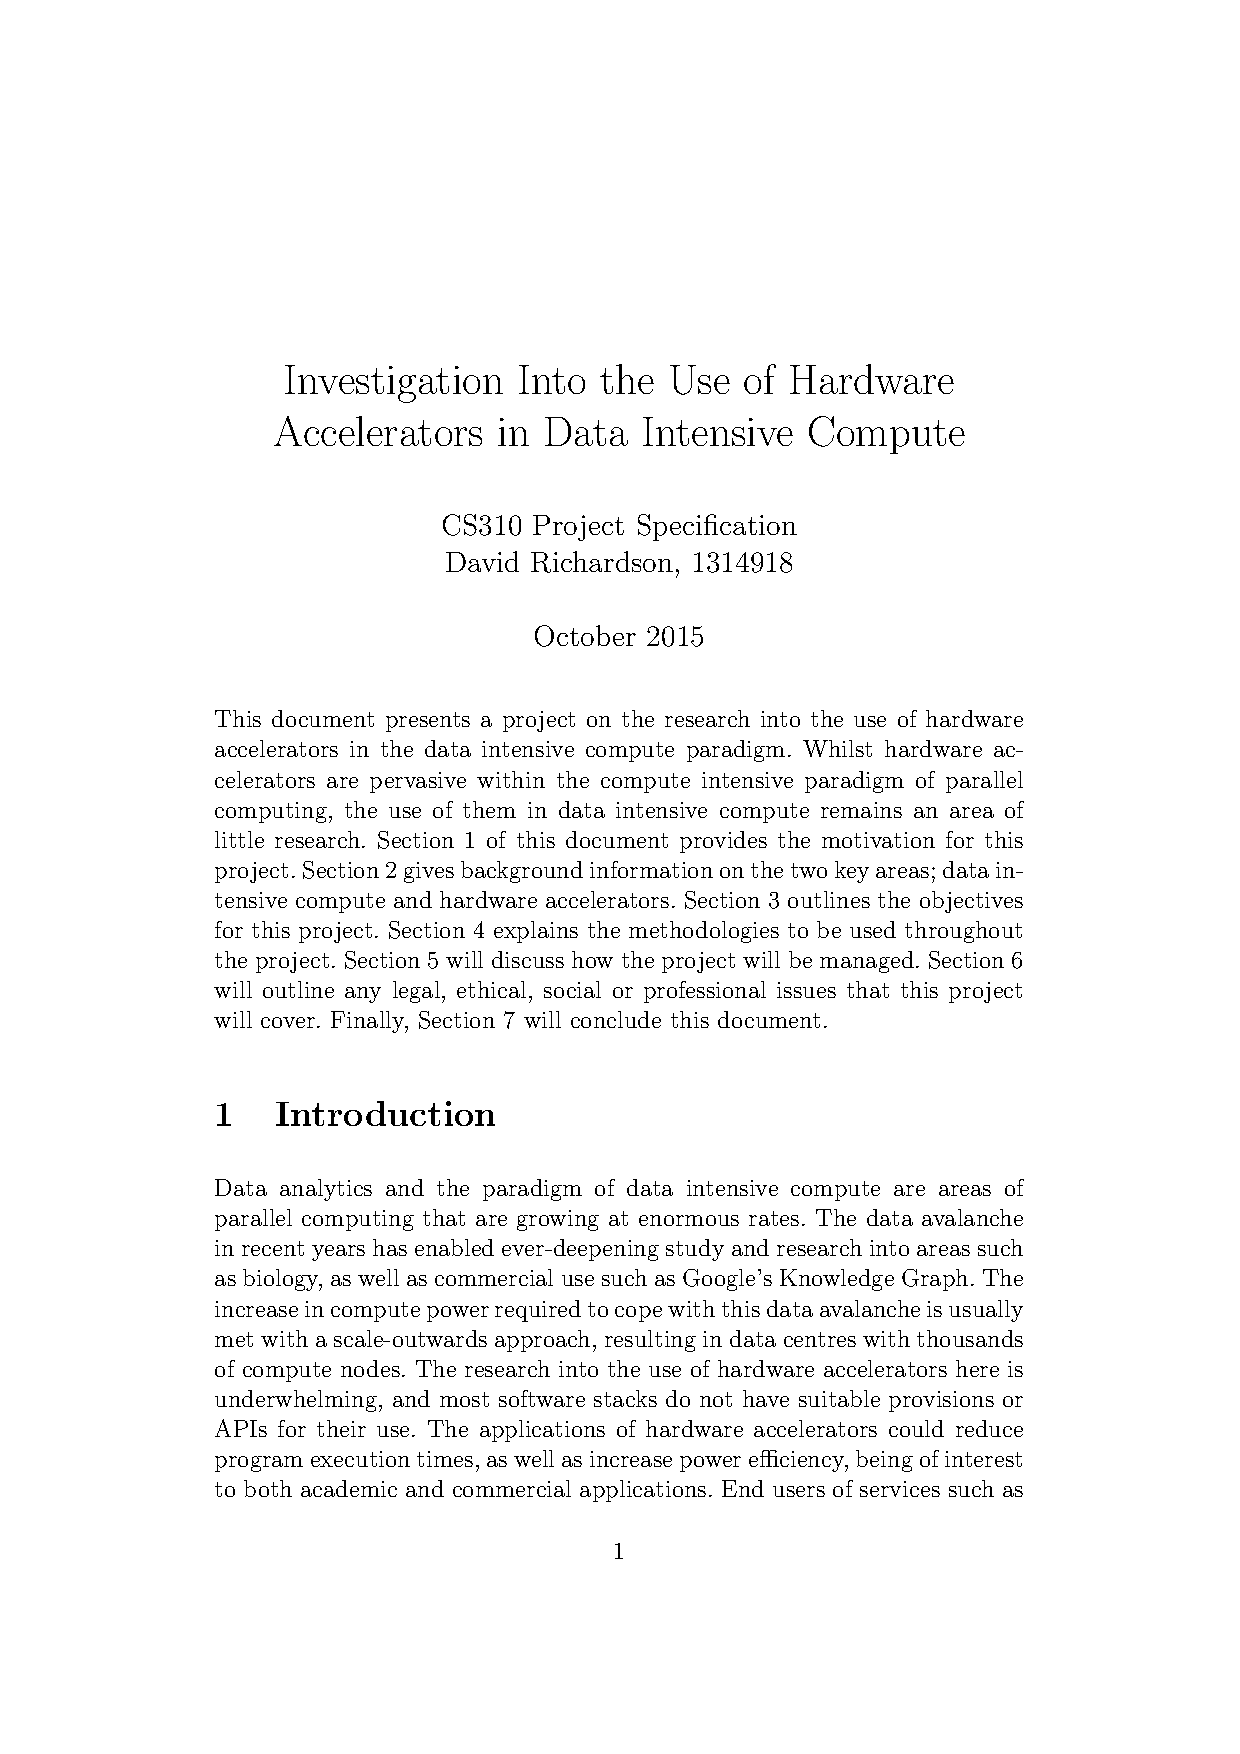
\includepdf[pages={1-12}, templatesize={16cm}{25.5cm}, frame=true]{specification.pdf}
	\end{appendix}

\end{document}